\documentclass{article}

\usepackage[utf8]{inputenc}
\usepackage[english]{babel}
 
\usepackage{multicol,caption}
%\usepackage{pgfplots}
\usepackage{graphicx}
\usepackage{footnote}
\makesavenoteenv{tabular}
\makesavenoteenv{figure}
\newenvironment{Figure}
  {\par\medskip\noindent\center\minipage{0.9\linewidth}}
  {\endminipage\par\bigskip\medskip}
  %figure inside multicols

\setlength{\oddsidemargin}{0pt}
% Marge gauche sur pages impaires
\setlength{\evensidemargin}{0pt}
% Marge gauche sur pages paires
\setlength{\textwidth}{470pt}
% Largeur de la zone de texte 
\setlength{\topmargin}{0pt}
% Pas de marge en haut
\setlength{\headheight}{13pt}
% Haut de page
\setlength{\headsep}{10pt}
% Entre le haut de page et le texte
\setlength{\footskip}{40pt}
% Bas de page + séparation
\setlength{\textheight}{630pt}
% Hauteur de la zone de texte 


\title{Micro-architectural Adaptation of Codelets using gem5 and CERE}
\author{Nicolas Derumigny \\
\small ENS de Lyon 
\and Pablo de Oliveira Castro\\ 
\small Université de Versailles Saint-Quentin-en-Yvelines}
\date{}


\begin{document}

\maketitle

\smallskip

\begin{abstract}
In recent years, many efforts have been deployed in order to increase the speed and efficiency of computing architectures. Another step to increase their efficiency is to adapt themselves to the tasks they do. For example, 64-bit computational power is not as useful as 16-bit one for neuronal network, so specific hardware, faster for 16-bit calculus but slower on 64-bit ones are being developed.

Heterogeneous multicore system, widely spread on embedded computing, already use two CPU cluster (big.LITTLE technology): the big cluster handles heavy tasks, and the little one, more power-efficient but slower, is used the rest of the time. Sometimes the different regions of an application fit better on some architecture, depending of the type of data and the operations they are dealing with. One the big.LITTLE architecture, they can be transferred from one cluster to the other during its running. 


The codelet approach, based on the use of the software Codelet Extractor and REplayer (CERE), allows to isolate and tune some sections of the application individually, showing which improvements on the hardware side leads to better performance. 


This report presents an overview of the possibility of micro-architectural adaptation using the x86 instruction set simulated by gem5, based on an performance-consumption ratio, calculated with MCPAT.
 Its impact has been measured on both sequential and parallel applications on one simulated monocore CPU, using the NAS and PARSEC benchmark suites. 
%comment result when they where

\end{abstract}



\begin{multicols}{2}

\section{Introduction}
\subsection{Generalities}
Developing a new CPU architectures is a compromise between several parameters. The common approach is to minimise the manufacturing cost and minimise the average execution time, measured on a suite of benchmark representative of the user's most frequent tasks. But in HPC, the needs depend mostly of the application run: for physicist calculus, a great precision is needed, so developing 128-bit compute units is needed. Whereas in deep learning machines, fast 16-bit computation is enough.

Thus, architectural adaptations could greatly improve the performance of computational unit executing only a fixed task. 

The boost technology, increasing the frequency during high loads while the chip is under a given temperature (or does not reach a thermal threshold) can also be taken as an on-the-fly tuning of some chips to adapt to a given task. An other example of this specialisation is GPGPUs and CPUs: GPGPU are efficient in highly-scalable parallel applications, and CPUs are faster on sequential ones.



\paragraph{}
CERE is a software that extracts fro; an application some pieces of codes corresponding to a selected region, called codelets. Extracted codelets presents themselves as another application that can be run out-of-the-box and recreates the behaviour of the selected region.


The gem5 simulator\cite{gem5-sim} has been used to quantify micro-architecture impacts on softwares: it allows to fine-tune parameters without using different processors. As it emulates a whole linux system, the measurement can be really slow, that is why running only codelets gives a serious advantage over measuring the entire application. For example, running the IS codelet is four times faster in SE mode that the full application.


\subsection{Experimental Protocol}
Four x86 CPUs were simulated, one based on the Cortex A-15\cite{DBLP:conf/samos/EndoCC14}, the i5-3550 (with turbo and non-turbo frequency), the i5-3770U, a low-power mobile CPU and a QX9100. All these CPUs are simulated as one-core CPU, using the one-core values for non-shared caches and real value for shared caches.

The codelets used were extracted using CERE\cite{CERE} tool, originally taken from NAS\cite{NAS} sequential benchmark suite and PARSEC\cite{PARSEC} benchmark suite. We chose NAS IS sequential as a simple serial application and pthread-disabled x264 for a more complicated one. Blackscholes and Freqmine, two OpenMP applications from PARSEC suite, were chosen to test multithread performance.


The energy consumption was computed using MCPAT\cite{MCPAT} and taken as a measure of the efficiency of each simulated CPU. Indeed, power consumption is the ideal measurement for architecture tuning, as it delimits on one side the maximum computational power of the CPU at fixed architecture (due to frequency limits) and on the other side the cost to run it.

This paper explains in section \ref{bckgrnd} the related work and its position comparing to the current research. Section \ref{sim} describes the compatibility between gem5 and the codelets extracted by CERE, along with the models, the values and the applications chosen for the simulations. Section \ref{results} demonstrates how CERE coupled with gem5 can be used to quickly tune heterogeneus architecture for each codelet.


\section{Background}
\label{bckgrnd}

\subsection{On the benchmarking of processors}
TODO/DELETE : Moreover, benchmarks are a good way to reproduce the usage of a computer\cite{select-bench}. %read this




\subsection{On the use of codelets}
% -------------- PICTURE ----------------
Source code isolation has already been validated as a reliable way to reproduce the comportement of applications. 

CERE is a software that creates \textit{codelets}, small parts of an application that can be run separately, from one loop of the application.
The loop run inside the application is called the \textit{in-vivo} codelet. CERE targets to create a copy of the original application running only this loop and recreating its execution (cache state especially should be as similar as possible). This process is called \textit{extraction} and leads to the \textit{in-vitro codelet}. The codelet running time is only the time taken by the loop to be executed; it does not include the memory restore stage and the cache warm-up sequence. 


CERE is a sofware that extracts codelets from a C/C++/Fortran application using the LLVM compiler. It operates at the Itermediare Represemtation (IR) level, and thus is more flexible than code isolation (isolating the codelet at the source-code level, then compile it) or assembly isolation (isolating the codelet at the binary file level)\cite{CERE}. 


At this time, CERE targets only loops and openMP parallel \textit{for} loops. On sequential NAS IS benchmark, the selected codelet covers more than 98\% of the total execution time, but is 7.3 to 46.6 times faster than running the full NAS.B suite.


CERE captures the memory context at a page-granularity level, which is lighter than a full dump and then faster to replace in memory when replaying inside a simulator. Moreover, a cache warm-up can done before replaying the codelet by running one time the selected loop. 
%or ????
This step should not be avoided when tuning microarchitecture parameters such as cache size or cache line size, as the warm-up could be slower but the other executions much faster.


\subsection{On the simulators}
\subsubsection*{The gem5 simulator}
The gem5 simulator is a cycle-accurate simulator. Its accuracy has been demonstrated on ARM simulation on both in-order and out-of-order processor, comparing real and simulated Cortex-A8 and Cortex-A9\cite{DBLP:conf/samos/EndoCC14}. This comparisons reveals an average absolute error of only 7\%.

Replaying SPLASH benchmark on gem5 shows an error on the execution time from 1.39\% to 17.94\%, explained by an inaccurate simulation of the DDR memory. Nevertheless, the gem5 simulator now handles different memory types, including modern DDR3, DDR4 and GDDR5, which should be more accurate than the tested DDR memory used in SPLASH tests\cite{DBLP:conf/recosoc/ButkoGOS12}.


\subsubsection*{The MCPAT simulator}
TODO or delete.


\section{Simulation framework}
\label{sim}

\subsection{The gem5 simulator}

The gem5 simulator can be run in two different modes: syscall emulation (SE) and fullsystem mode (FS). The Syscall emulation mode simulates only the behaviour of the CPU inside a linux operating system, and therefore cannot efficiently simulate multi-threaded application, as no scheduler has been implemented. Besides, SE mode required a static linkage of all the required libraries.

On the contrary, the fullsystem mode emulate a full CPU; as the OS is emulated, the simulation is really slow (about fifteen minutes to boot linux on an x86 AtomicSimpleCPU). Nevertheless, FS mode is more accurate and more flexible. Indeed, FS mode can handle dynamic libraries, assuming that they are well installed in the virtual disk image. 
Moreover, gem5 featured a checkpoint functionality which avoid booting again when the CPU is changed.


\subsubsection{Syscall emulation mode}
Two changes on gem5 has been made to allow the use of CERE sequential codelets. First, the \textit{getdents} syscall has been implemented, which is called inside the \textit{readdir} function, used in the codelet memory mapping function. The second change concern a bug occurring when reading EOF with the syscall \textit{read} while providing an invalid pointer: it should work and write nothing, but caused a page fault in gem5. Both patches were submitted to gem5 community.

\begin{Figure}
\centering
%%CHANGER LA LEGENDE "second"
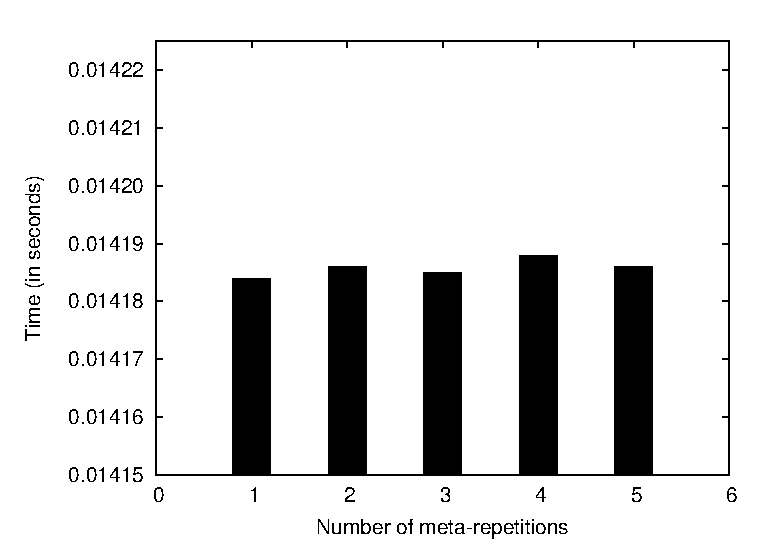
\includegraphics[width=\linewidth]{vari_se.eps}
\captionof{figure}{\label{vari_se}Variations of the codelet loop execution time on NAS IS class W benchmark using the i5-3550 configuration without turbo, with four CPUs.}
\end{Figure}


In order to statically compile codelets with CERE\footnote{CERE version 0.2 was used in this paper.}, the argument \textit{-static} must be provide at the link time. Noting that this could provoked some relocation error when specifying the entry point of the program: offset 0x60000000 (used as default start point in CERE) is used to place the standard C library in sequential NAS IS. Experimentally, offset 0x40000000 did not cause any trouble when compiling sequential codelets. 


OpenMP parallel codelets cannot be run on SE mode due to the lack of real pthread implementation in the SE subsystem. Indeed, statically linking with \textit{libiomp.a} results in a forced exit because of the missing pthread management syscalls.

\paragraph{}
With these changes, and assuming that all the syscalls have been implemented inside the gem5 simulator, any sequential codelet should work in SE mode. Given that there is no scheduler in gem5 SE mode, and given that there is no proper implementation of pthread implementation in SE mode\footnote{M5thread has not been tested due the lack of scheduler and the miss of important syscall implementations in SE mode.}, parallel codelets cannot be realistically replayed on SE mode.

\paragraph{}
Using the region \_\_cere\_\_is\_ranked\_475 with five meta-repetitions (six total runs of the loop, as one is used to warm the cache up), we observed 4x speedup, comparing to running the full benchmark\footnote{Class W inputs were used for all the results.}. All the data analysis is done on the median of these five meta-repetitions, but as the fluctuation is at most 0,03\% (figure \ref{vari_se})\footnote{This is due to the deterministic routine of the codelet, as the region \_\_cere\_\_is\_ranked\_475 is verifying that a give array is well-sorted. Such tight results are harder to get on randomised or multithreaded code, see section \ref{FS_mode}.}, we can imagine running a codelet with only two or three meta-repetitions without significant bias.

\subsubsection{Fullsystem mode}
\label{FS_mode}
To run codelets in FS mode, only a few changes have been done: a more recent image than the ubuntu 7.04 available on gem5 site has been used, base on ubuntu-core 14.04. The kernel used is version 3.2.40 with default gem5 configuration.


To run OpenMP applications, just putting the \textit{libiomp5.so} and \textit{libomp.so} in \textit{/usr/lib}\footnote{Taken from linux mint MATE 17.3 64 bits} works. Therefore setting KMP\_affinity to \textbf{scatter}, which should assign each thread to a different core if available, results in a segmentation fault when starting the codelet. As a consequence, codelets on small inputs shows inexploitable behaviour (figure \ref{freqmine_nogood}) on four cores.
%CHANGE THE FIGUUURRRRRREEEE "seconds" sans "e" !!!
 Moreover, gem5 seems to hang when simulating more than one x86 CPU in FS mode, that is why all the applications (including multicore's one) were run using a one-core configuration.

\subsection{Simulation models}
\subsubsection{Hardware configuration}
The chosen configurations are detailed in figure \ref{cpu_setup}. All systems are set with 8 GB of 1600 MHz DDR3, the cacheline size is always kept at 64 B, and all CPUs are quad-core without hyper-threading.

\subsubsection{Chosen codelets}
We chose three codelets to efficiently reproduce different usages:
\begin{itemize}
\item NAS IS sequential: region \_\_cere\_\_is\_ranked\_475 which check whether the computed array is sorted or not.
\item PARSEC\footnote{Version 3.0-beta-20150206} blackscholes: region \\ \_\_cere\_\_blackscholes\_m4\_\_Z9bs\_threadPv\_first, an OpenMP region calculating the option value based on the Black \& Scholes's equation.
\item PARSEC freqmine: region\\ \_\_cere\_\_tree8scan1\_DBEP4Data\_first which generates a hash from the tree dataset.
\item PARSEC x264: region \\ \_\_cere\_\_encoder\_analyse\_block\_residual\_write- \_cabac\_745 used in the CABAC encoding of the video.
\end{itemize}


\begin{Figure}
\centering
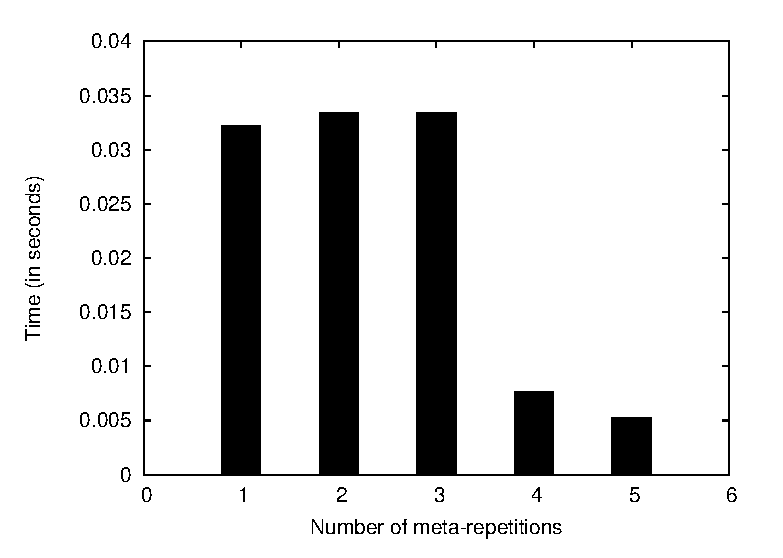
\includegraphics[width=\linewidth]{nogood.eps}
\captionof{figure}{\label{freqmine_nogood}Variations of the codelet loop execution time on PARSEC Freqmine benchmark using the Cortex-A15 configuration with four AtomicSimpleCPU and simtest input.}
\end{Figure}

\end{multicols}
\begin{figure}[ht]
\begin{center}

\begin{tabular}{| l | c | c | c | c | c | c |}
\hline 
& & & \multicolumn{2}{c|}{L2} &\\
Name & Frequency\footnote{Non-turbo - Turbo frequency when turbo techology is implemented} & L1D and L1I associativity\footnote{The L1D and L1I size is always 32 kB.} & Size & Assoc. & L3 \\
\hline

Cortex-A15 & 1 GHz & 2 & 1 MB & 16 & No \\

i5-3550 & 3,3-3,7 GHz & 8 & $4 \times 256$ kB & 8 & Yes\footnote{The size of the L3 cache is set to 8MB and its associativity to 16-way due to gem5 limitations, it should be 6MB and 12-way.}\\

i5-3337U & 1,8-2,7\footnote{Only the non-turbo frequency has been simulated} GHz & 8\footnote{It should be 6 MB.} & $4 \times 256$ kB & 16 & Yes\footnote{It should be 3 MB.}\\

Q9100 & 2,26 GHz & 8 & 8 MB\footnote{It should be 6 MB and 12-way.} & 16 & No\\



\hline

\end{tabular}
\caption{\label{cpu_setup}Parameters used for CPU simulations.}
\end{center}
\end{figure}
\begin{multicols}{2}

\section{Results}
\label{results}
The power consumption of each CPU is calculated roughly using gem5 output file by the MCPAT software: such value should not be taken absolutely but relatively to other CPU simulated. A power consumption of 10W is indeed too small for an one-core X86 desktop CPU running a benchmark. 

One have to keep in mind that the CPUs use only using a generic x86 scheme, without hyper-threading or other technological improvements (pipeline aside), and own only one core. That is why only relative measured at fixed codelets are really meaningful.

\subsection{Power/performance ratio and index}
The performance of a CPU is measured by the execution time of the selected codelet. To keep an higher-is-better index, only $1/t_e$ values are used (where $t_e$ is the execution time).
The power-comsumpution ratio is defined as 
\begin{equation}
\frac{1}{P.t_e}
\end{equation}
With $P$ the power consumption of the CPU on the benchmark.

A higher ratio means either better performance or less comsumption, and so a better choice.


\subsubsection{IS : A serial applications}
\begin{Figure}
\centering
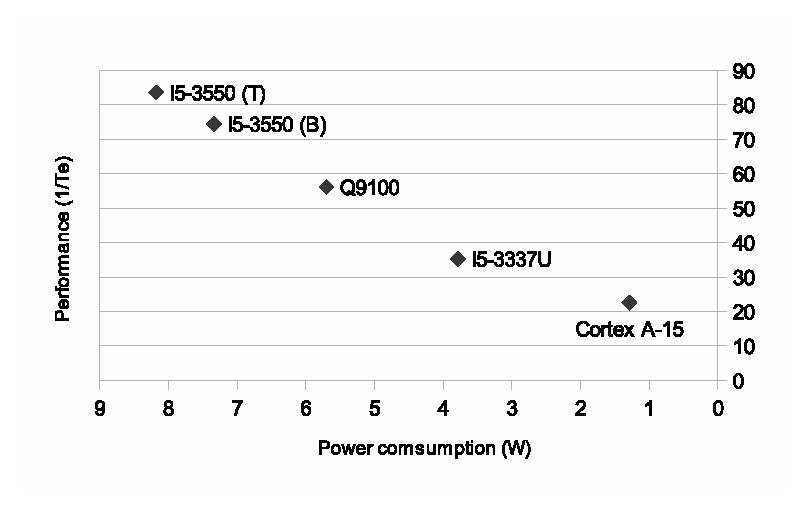
\includegraphics[width=\linewidth]{IS.eps}
\captionof{figure}{\label{IS}Power-Performance graph for the IS codelet.}
\end{Figure}

\begin{Figure}
\centering
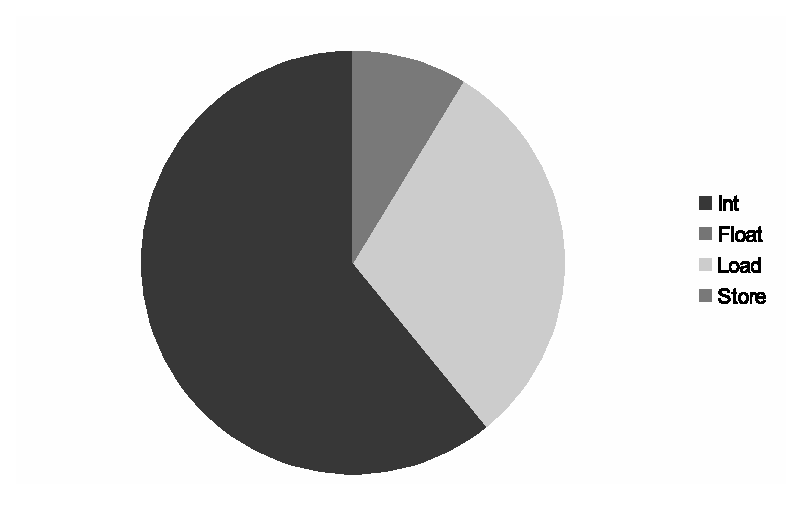
\includegraphics[width=\linewidth]{IS_instr.eps}
\captionof{figure}{\label{IS_instr}Repartition of the instructions during the execution of the IS codelet.}
\end{Figure}


\paragraph{x264\\}
?


\subsubsection{Parallel applications}
This parallel applications are run on a one-core configuration: these results are only bound to show the single-core performance-consumption differences, and not the manycore scaling. Such studys could easily be measured on ARM systems (see \ref{ARM_sim}).

\paragraph{Freqmine\\}
Freqmine was tested with a small data input. Therefore, all data can fit in cache. The Q9100 L2 cache is faster than the i5-3350 L3 cache, so the former is slightly faster than the latter at stock frequency on this benchmark - but consumes much regards to the improvement (figure \ref{Freq}). With the turbo enabled, the i5-3550 stays first.

\begin{Figure}
\centering
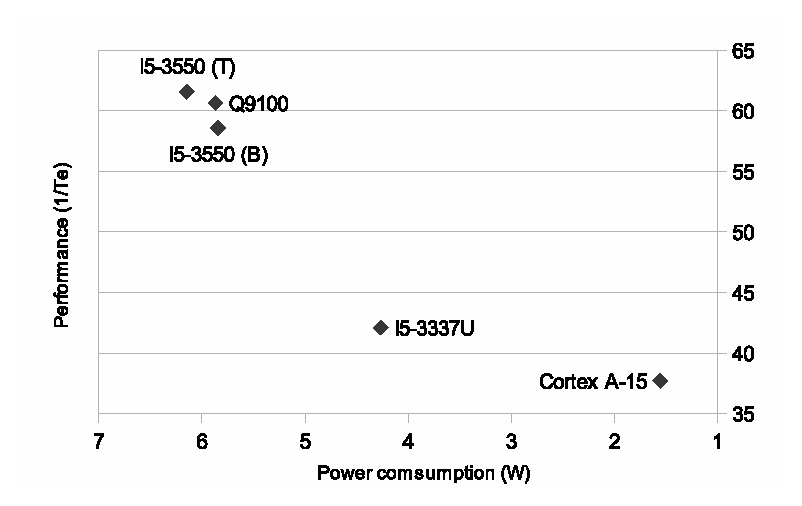
\includegraphics[width=\linewidth]{Freqmine.eps}
\captionof{figure}{\label{Freq}Power-Performance graph for the Freqmine codelet.}
\end{Figure}

\begin{Figure}
\centering
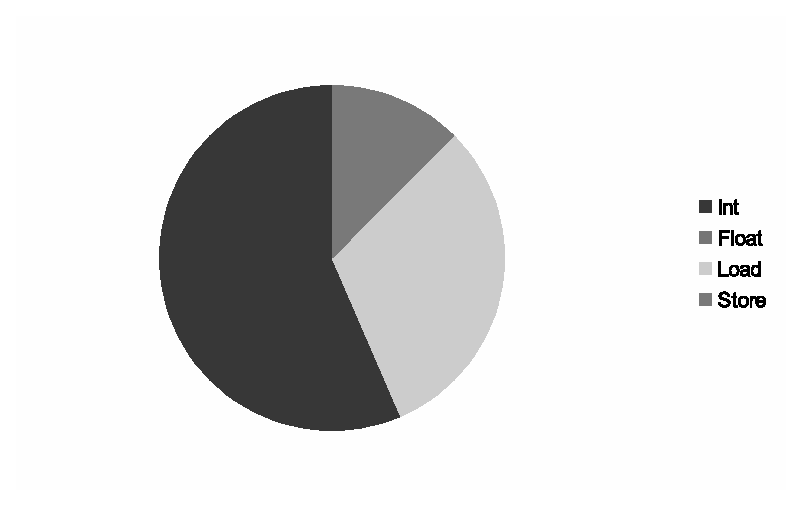
\includegraphics[width=\linewidth]{Freqmine_instr.eps}
\captionof{figure}{\label{Freq_instr}Distribution of the instructions during the execution of the Freqmine codelet.}
\end{Figure}


\paragraph{Blackscholes\\}
\label{Blackscholes}

\begin{Figure}
\centering
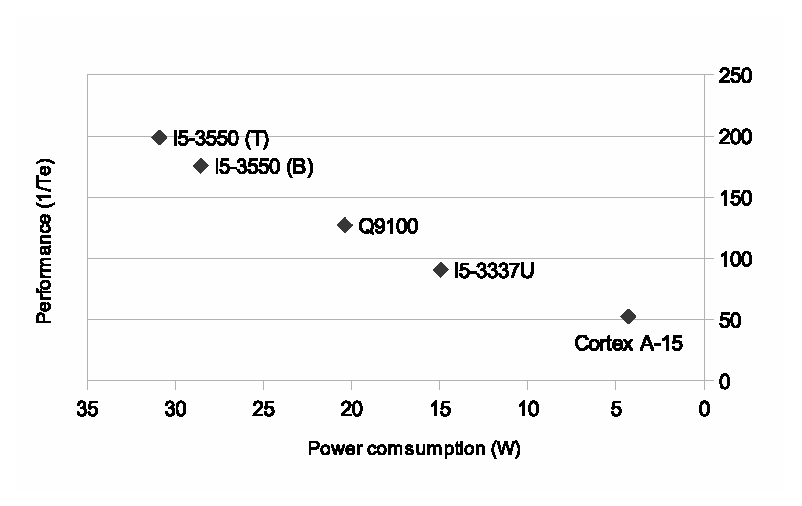
\includegraphics[width=\linewidth]{Blackscholes.eps}
\captionof{figure}{\label{Blasch}Power-Performance graph for the Blackscholes codelet.}
\end{Figure}

\begin{Figure}
\centering
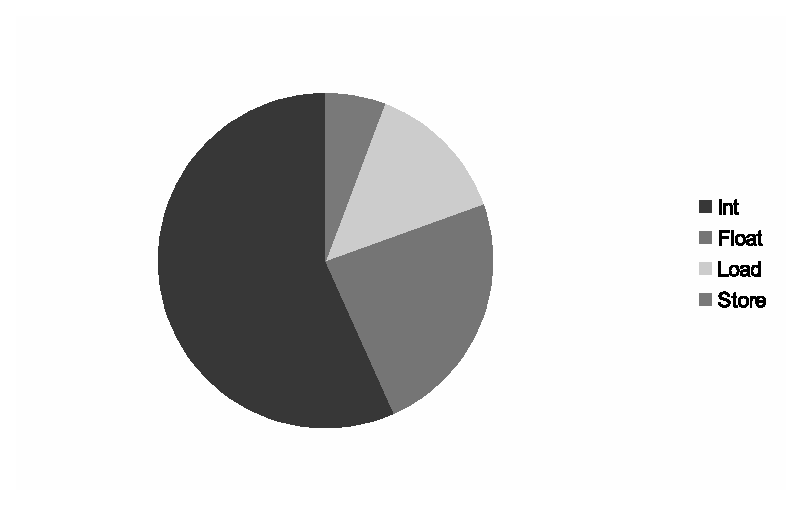
\includegraphics[width=\linewidth]{Blackscholes_instr.eps}
\captionof{figure}{\label{Blasch_instr}Distribution of the instructions during the execution of the Blackscholes codelet.}
\end{Figure}

\subsection{Performance}
\begin{Figure}
\centering
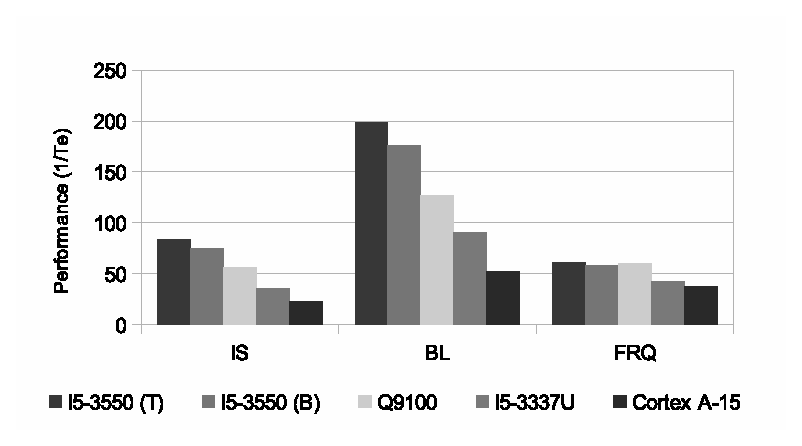
\includegraphics[width=\linewidth]{Performance.eps}
\captionof{figure}{\label{Perf}Performance of all tested CPUs on differents codelets.}
\end{Figure}


X264 codelet is too fast too measure the execution time with gem5 (only 0,0000001 or 0,0000002 seconds are calculated), so this codelet will only be analysed for its power consumption.


IS and freqmine does execute on the same order of time (figure \ref{Perf}), even if freqmine codelet was extracted running the simtest input. 



\subsection{Power consumption}
When the power consumption is on the $x$ axis, the former is graduated backward to keep and higher-is-better index.


\begin{Figure}
\centering
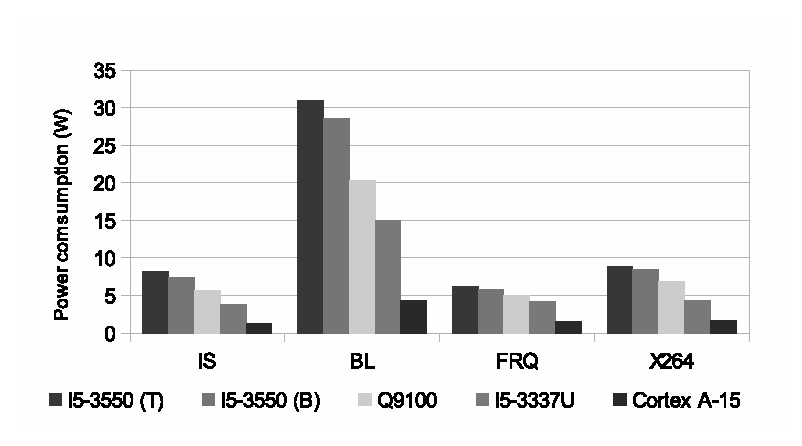
\includegraphics[width=\linewidth]{Power_consumption.eps}
\captionof{figure}{\label{Pow}Power consumption for each CPU.}
\end{Figure}

For example, the blackscholes codelets seems to consume more power than all the other codelets (figure \ref{Pow}). This is due to floating point operations, used significantly only in this codelet (see \ref{Blackscholes}).


\begin{Figure}
\centering
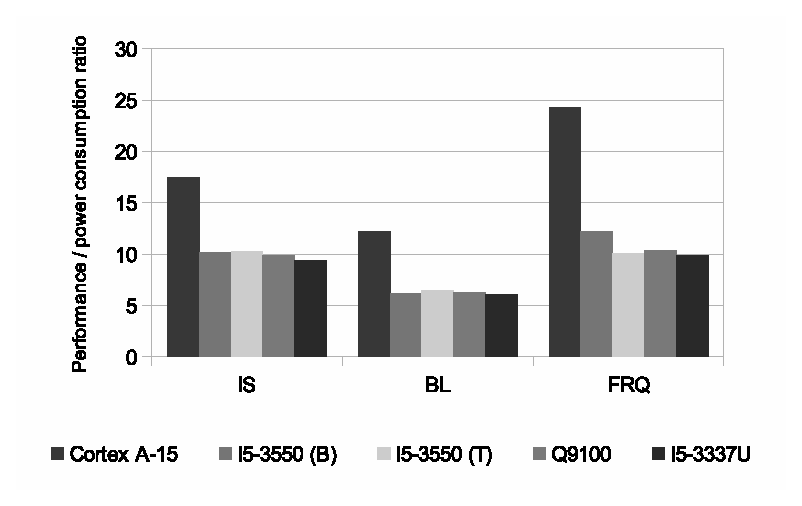
\includegraphics[width=\linewidth]{Ratio.eps}
\captionof{figure}{\label{Ratio}Performance-Power consumption ratio for each codelets.}
\end{Figure}

\subsection{Advantages}
The use of codelets gives a powerful tool to fine-tune the architecture fitting to the codelets. Because of CERE limitations, only codelets replay \textit{for} loops or \textit{omp parallel for} loops are supported, but this is much lighter than running the full application. Moreover, codelets can improve individually each region of an application, which is extremely useful to choose on which CPU cluster run the application on a big.LITTLE system, or even in an heterogeneus compute server.

The gem5 simulator is a precise tool to reproduce the behaviour of a specific machine on a general computer. As the simulation is quite slow, the use of codelets could be really useful in term of time and resources in the conception of heterogeneous servers. As CERE operates as an IR-level, the operation does not need any additional work on the source code, and can be run in C, C++ or Fortran programs. Besides, the compilation of the codelets uses the power of the host machine and not the simulated one, which is really useful in term of compute time: the emulated system is used only when it is truly needed.

\subsection{Inconvenient : Unknown precision}
Gem5 is a simulator, and therefore cannot be entirely trusted. CERE too cannot exactly replay a whole execution of an application ; and the measures output by MCPAT are only an estimation of the effective power consumption of the CPUs: that's why the results could not fit exactly to the real-life experiments. Nevertheless, these simulations are bound to give an overview of the gains that could be archived by improving a specific part of a CPU, not to give absolute results.

The gem5 simulator has not been validated yet on x86 accuracy, and could be quite biased, as it emulates a generic x86 processor, whereas state of the art CPUs are even more complex.


\section{Conclusion}
\label{ccl}
To our knowledge, no other work has been produced before using codelets to do architectural-tuning inside a simulator.
TODO

\newpage

\bibliographystyle{plain}
\bibliography{report}


\newpage
\section{Annexe}
\subsection{ARM Simulation}
\label{ARM_sim}
As multicore benchmarks seem to hang on X86 simulation, some work has been done to adapt the codelet on ARM simulation.
The multicore simulation works with linaro-minimal

As capturing on ARM required an ARM machine, a few cross-compile instructions has been added in CERE. Capturing en gem5 may indeed take several days, and require moreover an ARM version of CERE pre-installed on the virtual machine, which is too heavy to be implemented yet. The goal is then to use an x86 memory dump and replay it on ARM systems. The following changes have been made in CERE:
\begin{itemize}
\item Changed objdump to aarch64-linux-gnueabi-objdump.
\item Added clang cross-compile option.
\end{itemize}

After thoses changed, the compilation ran successfully, but the execution outputs \textit{"Killed"}, even before the main() starts.


We found that the aarch64 architecture limits the application space to the address 0x00000000\_00000000 to 0x0000ffff\_ffffffff\cite{aarch64-mmu}.
%PUT A PICTURE !!!!!
 But the stack is placed on x86 linux at address 0x07fda3c7\_b0000000 so the kernel kills the application as soon as the X86 stack region is reserved.
To avoid this issue, the stack has manually been moved to address 0x000003c7\_b0000000.

NAS IS (codelet \_\_cere\_\_is\_ranked\_475) has been successfully replayed on a juno board (linaro-image-minimal-genericarmv8 system) using this trick. Nevertheless, further adaptations have to be done in order to safely convert x86 dumps to ARM dumps\footnote{Especially on pointers of stack address which need to be updated to the new stack position at the codelet compilation.}.


\subsection{About the UVSQ laboratory}
%see the report instruction on the web

\subsection{Gem5 patches}

\end{multicols}

\end{document}